\documentclass[aps,prxquantum,preprint,superscriptaddress,amsmath,amssymb]{revtex4-2}
\usepackage{graphicx}
\graphicspath{{./figures/}}
\usepackage{bm}
\usepackage{siunitx}
\usepackage{xcolor}
\usepackage{booktabs}
\usepackage{braket}
\usepackage[colorlinks=true, citecolor=blue, linkcolor=blue, urlcolor=blue]{hyperref}
\usepackage{xr-hyper}
\usepackage[capitalize, nameinlink]{cleveref}
\externaldocument[MAIN-]{main}
% --- Track C shared setup (siunitx, notation macros, cleveref names) ---
\sisetup{
  retain-unity-mantissa = false,
  exponent-product = \times
}
\setlength{\emergencystretch}{1.5em}
\DeclareSIUnit{\dB}{\deci\bel}

% --- Notation macros (identical in main text and Supplemental Material) ---
\providecommand{\mel}[3]{\langle #1 \vert #2 \vert #3 \rangle}
\providecommand{\ev}[1]{\langle #1 \rangle}
\newcommand{\Real}{\operatorname{Re}}
\newcommand{\Tr}{\operatorname{Tr}}
\newcommand{\Fnorm}{F_C^{\rm norm}}
\newcommand{\Fnormeff}{F_C^{\rm norm,eff}}
\newcommand{\Fraw}{F_C^{\rm raw}}
\newcommand{\Gfwd}{G_{\rm fwd}}
\newcommand{\Grev}{G_{\rm rev}}
\newcommand{\Iso}{\mathcal{I}}
\newcommand{\gNR}{\gamma_{\rm NR}}
\newcommand{\lint}{\lambda_{\rm inter}}

% --- cleveref: consistent, spelled-out cross-reference names ---
\crefname{equation}{Eq.}{Eqs.}
\Crefname{equation}{Equation}{Equations}
\crefname{table}{Table}{Tables}
\crefname{figure}{Fig.}{Figs.}
\Crefname{figure}{Figure}{Figures}
\crefname{section}{Sec.}{Secs.}

\renewcommand{\theequation}{S\arabic{equation}}
\setcounter{equation}{0}
\renewcommand{\thefigure}{S\arabic{figure}}
\setcounter{figure}{0}
\renewcommand{\thetable}{S\arabic{table}}
\setcounter{table}{0}
\renewcommand{\thesection}{S\arabic{section}}
\renewcommand{\thesubsection}{S\arabic{section}.\arabic{subsection}}

\begin{document}

\title{Supplemental Material for ``Spatial channel separation evades the single-port Petermann bound in a non-Hermitian optomechanical ladder''}

\author{Juste Deuyekbe}
\affiliation{Department of Physics, Faculty of Science, University of Ngaoundere, P.O. Box 454, Ngaoundere, Cameroon}

\author{P. Djorw\'e}
\email{djorwepp@gmail.com}
\affiliation{Department of Physics, Faculty of Science, University of Ngaoundere, P.O. Box 454, Ngaoundere, Cameroon}
\affiliation{Stellenbosch Institute for Advanced Study (STIAS), Wallenberg Research Centre at Stellenbosch University, Stellenbosch 7600, South Africa}

\author{A.-H. Abdel-Aty}
\affiliation{Department of Physics, College of Sciences, University of Bisha, Bisha 61922, Saudi Arabia}

\author{A. Elrashidi}
\email{a.elrashidi@ubt.edu.sa}
\affiliation{College of Engineering, University of Business and Technology, Jeddah 21448, Saudi Arabia}

\author{Nsangou Mama}
\email{mnsangou@yahoo.com}
\affiliation{Department of Physics, Faculty of Science, University of Maroua, P.O.Box 46, Maroua, Cameroon}

\author{S. G. Nana Engo}
\email{serge.nana-engo@facsciences-uy1.cm}
\affiliation{Department of Physics, Faculty of Science, University of Yaounde I, P.O.Box 812, Yaounde, Cameroon}

\maketitle

This Supplemental Material provides the theoretical framework (\cref{sec:si_theory}), the single-chain benchmark (\cref{sec:si_single}), the double-chain ladder parameters and solution classes (\cref{sec:si_double}), the disorder-resilience study (\cref{sec:si_disorder}), the initialization-resampling characterization (\cref{sec:si_seed_dependence}), the OTOC and cutoff-convergence diagnostics (\cref{sec:si_otoc}), the weak-force and axion projections (\cref{sec:si_apps}), and the scope boundaries (\cref{sec:si_limitations}).

\section{Theoretical framework}
\label{sec:si_theory}

The non-Hermitian tight-binding Hamiltonian for a one-dimensional cavity array with asymmetric hopping is
\begin{equation}\label{eq:si_nhse}
\hat{H}_{\rm NH}=\sum_{j=1}^{N}\bigl(J e^{g}\hat{c}_{j+1}^{\dagger}\hat{c}_{j}+\,J e^{-g}\hat{c}_{j}^{\dagger}\hat{c}_{j+1}\bigr),
\end{equation}
where $g$ is the logarithmic hopping asymmetry and $J$ the bare nearest-neighbor hopping amplitude~\citep{Yao2018,Hatano1997}. The non-reciprocal rate is $\gNR=2J\sinh(g)$, and the operating criterion for skin-mode localization is $\gNR/\kappa\ge\num{2}$~\citep{Bergholtz2021,Schomerus2020}.

Under open boundary conditions (OBC) the single-particle drift matrix takes the form
\begin{align}\label{eq:si_obc_drift}
&A_{jj}=-\kappa,
&&A_{j+1,j}=J e^{g},
&A_{j,j+1}=J e^{-g}.
\end{align}
The corresponding right and left skin-mode profiles are
\begin{align}\label{eq:si_skin}
&r_{n,j}\propto e^{g j}\sin\Bigl(\frac{n\pi j}{N+1}\Bigr),
&\ell_{n,j}\propto e^{-g j}\sin\Bigl(\frac{n\pi j}{N+1}\Bigr).
\end{align}

Time evolution of the open optomechanical density matrix is evaluated using the Duhamel variation-of-constants integral formula
\begin{equation}\label{eq:si_duhamel}
\rho(t) = e^{\mathcal{L}t}\rho(0) + \int_0^t e^{\mathcal{L}(t-s)}\mathcal{D}[\rho(s)]\, ds,
\end{equation}
where $\mathcal{L}$ is the reference unperturbed Liouvillian superoperator and $\mathcal{D}$ the dissipative or non-Hermitian coupling perturbation. Restricting evaluations to the Lyapunov window $t<1/\lambda_{\max}$ ensures that linear error growth remains strictly bounded; this bound motivates restricting the OTOC fits of \cref{sec:si_otoc} to the early-time window $t\in\numrange{0.5}{1.5}\,\kappa^{-1}$, before the perturbative expansion underlying \cref{eq:si_duhamel} breaks down.

Array phase stabilization is achieved via synthesized Kuramoto phase-locking potentials
\begin{equation}\label{eq:si_kuramoto}
\dot{\theta}_j = \omega_j + \sum_k K_{jk} \sin(\theta_k - \theta_j),
\end{equation}
where $\theta_j$ represents the mechanical resonator phase and $K_{jk}$ denotes the synthesized inter-site coupling matrix. The nonlinear synchronization term locks the relative phase of the two chains at whichever value $\phi_{\rm opt}(N)$ the DOC optimizer selects for a given size; these optimized phases range over $\phi\in\numrange{1.35}{5.15}\,\mathrm{rad}$ across the six solutions of \cref{tab:si_nscaling} and do not cluster near a single chiral point. A fixed $\phi=\pi/2$ is imposed only in the dedicated disorder-resilience reference configuration of \cref{sec:si_disorder}, where it is a design choice of that study rather than a DOC output. Without this locking, thermal crosstalk and slow drift would detune $\phi$ away from its optimized operating value. Experimental drive schemes for setting and holding $\phi$ (auxiliary parametric electro-optic modulation or phase-locked sideband pumps) are detailed in \cref{sec:si_evanescent}.

The biorthogonal quantum Fisher information (QFI) for non-Hermitian systems is~\citep{Yao2018}
\begin{equation}\label{eq:si_biorth_qfi}
\mathcal{I}_Q(\theta) = \sum_{n,m} \frac{|\mel{\psi_n^L}{\partial_\theta \hat{H}_\theta}{\psi_m^R}|^2}{(\gamma_n - \gamma_m)^2 + (\epsilon_n - \epsilon_m)^2},
\end{equation}
where $\ket{\psi_n^{R}}$ and $\ket{\psi_n^{L}}$ denote the right and left eigenvectors with complex eigenvalues $\gamma_n - i\epsilon_n$. Near exceptional points the denominator vanishes, producing numerical gradient singularities during optimization.

The Petermann factor of mode $n$ is~\citep{Zhang2019,Caves1982}
\begin{align}\label{eq:si_petermann}
&K_n^{\rm raw}=\frac{1}{|\Braket{\ell_n|r_n}|^2},
&K_n^{\rm floor}=\frac{1}{\max\{|\Braket{\ell_n|r_n}|,\varepsilon\}^2},
\qquad \varepsilon=\num{1e-12}.
\end{align}
The numerical floor $\varepsilon=\num{1e-12}$ is a computational safeguard that prevents division-by-zero in automatic differentiation near exceptional points; it does not represent a physical noise floor~\citep{Bergholtz2021}. At the converged operating points the biorthogonal overlap is $\approx\num{0.96}\gg\varepsilon$, so the regularized and unregularized Petermann factors coincide ($K_{\rm eff}=K_{\rm raw}$). The floor is only active during gradient descent when the optimizer traverses regions near exceptional rings ($K\sim\num{1e14}$); once the optimizer converges to the NHSE phase, the floor is irrelevant.

\Cref{tab:si_petermann_sensitivity} confirms that $K_{\rm eff}$ is insensitive to the choice of $\varepsilon$ over eight orders of magnitude.

\begin{table}[hbtp]
\centering
\caption{Sensitivity of the regularized Petermann factor $K_{\rm eff}$ to the regularization floor $\varepsilon$ at a representative operating point ($J=\qty{0.138}{\kappa}$, $g=\num{2.055}$, $\lint=\qty{0.010}{\kappa}$, $\phi=\num{1.736}$), distinct from the six DOC-optimized configurations of the $N$-scan reported in \cref{tab:si_nscaling}.}
\label{tab:si_petermann_sensitivity}
\begin{tabular}{S S}
\toprule
{$\varepsilon$} & {$K_{\rm eff}$} \\
\midrule
1e-8  & 1.04 \\
1e-10 & 1.04 \\
1e-12 & 1.04 \\
1e-14 & 1.04 \\
1e-16 & 1.04 \\
\bottomrule
\end{tabular}
\end{table}

\section{Single-chain baseline: matched SNR and Fisher scaling}
\label{sec:si_single}

For a single open-boundary chain driven at one port, the stationary covariance under vacuum noise satisfies the continuous Lyapunov equation
\begin{equation}
AV+VA^{\dagger}+2\kappa\mathbb{I}=0,
\end{equation}
and the matched boundary signal-to-noise ratio is
\begin{equation}\label{eq:si_matched_snr}
\mathrm{SNR}_N = \frac{s_N}{V_{NN}} = \frac{|[-A^{-1}]_{N1}\Delta\theta|^2}{V_{NN}},
\end{equation}
where $s_N=|[-A^{-1}]_{N1}\Delta\theta|^2$ is the boundary signal power and $V_{NN}=[V]_{NN}$ the boundary Lyapunov noise variance. The continuous Gaussian homodyne measurement-record Fisher information at phase quadrature $\pi/2$ decomposes as~\citep{Radaelli2023}
\begin{equation}\label{eq:si_fisher_decomposition}
F_C = F_{\rm mean}+F_{\rm cov} = (\partial_\theta\bm{\mu})^T\Sigma^{-1}(\partial_\theta\bm{\mu}) + \frac12 \Tr\!\left[(\Sigma^{-1}\partial_\theta\Sigma)^2\right],
\end{equation}
combining mean-response and covariance-derivative terms. Data are reported for $N\in\{\numlist{6;8;10;12;14;16}\}$ at $J=\qty{0.5}{\kappa}$, $g=\num{1.7}$ ($\gNR/\kappa=\num{2.646}$).

\begin{table}[hbt]
\centering
\caption{Single-chain matched SNR and Fisher information in the target NHSE regime. All sizes are Hurwitz-stable ($\max\Real\lambda<0$).}
\label{tab:si_single}
\resizebox{\columnwidth}{!}{%
\begin{tabular}{S S S S S S S S}
\toprule
{$N$} & {$\max\Real\lambda$} & {$s_N$} & {$V_{NN}$} & {$\mathrm{SNR}_N$} & {$\Fraw$} & {$\|\mu\|^2$} & {$\Fnorm$} \\
\midrule
6  & -0.0990 & 1.972e0  & 1.665e5  & 1.184e-5 & 1.086e4  & 2.195e6  & 4.947e-3 \\
8  & -0.0603 & 1.071e3  & 5.542e7  & 1.932e-5 & 9.758e5  & 1.189e9  & 8.204e-4 \\
10 & -0.0405 & 6.437e5  & 2.247e10 & 2.864e-5 & 1.177e8  & 7.139e11 & 1.649e-4 \\
12 & -0.0291 & 4.138e8  & 1.039e13 & 3.981e-5 & 1.708e10 & 4.584e14 & 3.725e-5 \\
14 & -0.0219 & 2.791e11 & 5.282e15 & 5.283e-5 & 2.481e12 & 3.089e17 & 8.032e-6 \\
16 & -0.0170 & 1.951e14 & 2.881e18 & 6.771e-5 & 5.336e14 & 2.158e20 & 2.472e-6 \\
\bottomrule
\end{tabular}%
}
\end{table}

Semi-log fits over $N\in[6,16]$ give
\begin{align}
a_{\rm snr}&=+\num{0.1723}\quad(R^2=\num{0.9843}),\\
a_{\rm raw}&=+\num{2.4616}\quad(R^2=\num{0.9992}),\\
a_{\rm norm}&=-\num{0.7625}\quad(R^2=\num{0.9964}).
\end{align}
The negative resource-normalized slope recovers the single-port bound of Lau and Clerk~\citep{Lau2018} and of McDonald and Clerk~\citep{McDonald2020}: internal photon occupancy grows faster than the Fisher information. At fixed $(J,g)=(\num{0.5}\kappa,\num{1.7})$, the single-chain benchmark yields $\Fnorm\approx\num{3.7e-5}$ at $N=\num{12}$, three orders of magnitude below the double-chain marginal class.

\begin{figure}[htpb]
\centering
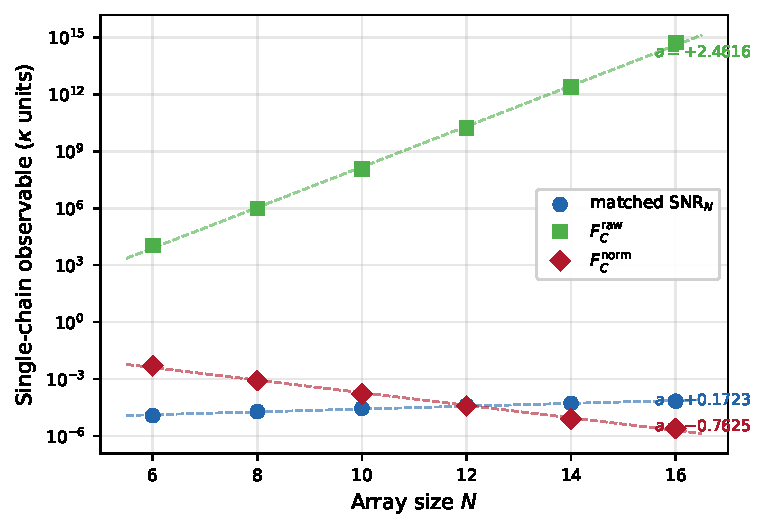
\includegraphics[width=0.8\columnwidth]{nhse_vs_ep_scaling.pdf}
\caption{Single-chain baseline scaling at fixed $(J,g)=(\num{0.5}\kappa,\num{1.7})$: the matched boundary SNR ($a_{\rm snr}=+\num{0.1723}$) and the raw record Fisher information ($a_{\rm raw}=+\num{2.4616}$) grow exponentially with $N$, while resource normalization reverses the trend ($a_{\rm norm}=-\num{0.7625}$): internal photon accumulation outpaces the Fisher gain, realizing the single-port resource bound.}
\label{fig:si_nhse_vs_ep}
\end{figure}

\section{Double-chain ladder: N-scaling and solution classes}
\label{sec:si_double}

The total non-Hermitian tight-binding Hamiltonian for the ladder array is~\citep{McDonald2020Exponential}
\begin{equation}
\hat{H}_{\rm ladder} = \hat{H}_A + \hat{H}_B + \hat{H}_{\rm inter},
\end{equation}
with the individual chain Hamiltonians and inter-chain coupling
\begin{align}
\hat{H}_A &= \sum_{j=1}^{N-1}\!\bigl(J e^{+g}\hat{a}_{j+1}^\dagger\hat{a}_j + J e^{-g}\hat{a}_j^\dagger\hat{a}_{j+1}\bigr) + \theta\,\hat{a}_N^\dagger\hat{a}_N, \label{eq:si_ladder_ha}\\
\hat{H}_B &= \sum_{j=1}^{N-1}\!\bigl(J e^{-g}\hat{b}_{j+1}^\dagger\hat{b}_j + J e^{+g}\hat{b}_j^\dagger\hat{b}_{j+1}\bigr), \label{eq:si_ladder_hb}\\
\hat{H}_{\rm inter} &= \sum_{j=1}^{N}\!\bigl(\lint e^{i\phi}\hat{b}_j^\dagger\hat{a}_j + \lint e^{-i\phi}\hat{a}_j^\dagger\hat{b}_j\bigr). \label{eq:si_ladder_hinter}
\end{align}
Chain~A has $\gNR^{(A)}=2J\sinh(g)\ge\num{2.0}\kappa$ (skin modes toward $j=N$), while chain~B has inverted hopping ($\gNR^{(B)}=-2J\sinh(g)$), driving skin modes toward $j=1$. This spatial segregation assigns chain~A as the sensing arm and chain~B as the noise-drain arm.

The joint drift matrix of the ladder is
\begin{equation}
A_{\rm ladder}(\theta)=\begin{pmatrix}A_A(\theta)&\Lambda\\\Lambda^\dagger&A_B\end{pmatrix},
\end{equation}
with opposing non-reciprocity on the two chains and inter-chain coupling $\Lambda=\lint e^{i\phi}\mathbb{I}_N$. Resource normalization counts photons on both chains. Directional gain is obtained from the scattering matrix $S=\mathbb{I}-\sqrt{2\kappa}\,A_{\rm ladder}^{-1}$.

Differentiable optimal control (Adam, 500 iterations, 5 random restarts, stability barrier $\max\Real\lambda<\num{-0.05}$)~\citep{Leung2017} produces the performance summarized in \cref{tab:si_nscaling}.

\begin{table}[hbt]
\centering
\caption{Double-chain DOC results across system size. Isolation $\Iso=\Gfwd-\Grev$. All entries satisfy $\max\Real\lambda<\num{-0.05}$.}
\label{tab:si_nscaling}
\begin{tabular}{S S S S S S S S}
\toprule
{$N$} & {$J/\kappa$} & {$g$} & {$\lint/\kappa$} & {$\phi$~[rad]} & {$\Fnorm$} & {$\Gfwd$~[\si{\dB}]} & {Isolation~[\si{\dB}]} \\
\midrule
6  & 0.105 & 1.250 & 0.0164 & 4.029 & 0.937 & -40.1  & 69.6 \\
8  & 0.354 & 0.973 & 0.0695 & 2.048 & 0.101 & +13.5  & 40.5 \\
10 & 0.078 & 1.001 & 0.0790 & 3.863 & 0.984 & -117.3 & 41.5 \\
12 & 0.345 & 1.024 & 0.0278 & 4.726 & 0.050 & +15.5  & 56.9 \\
14 & 0.087 & 0.797 & 0.0775 & 1.347 & 0.987 & -181.3 & 40.4 \\
16 & 0.287 & 1.226 & 0.0207 & 5.150 & 0.043 & +14.3  & 64.0 \\
\bottomrule
\end{tabular}
\end{table}

Two classes appear:

\begin{itemize}
\item \textbf{Deep-stability} ($N=\numlist{6;10;14}$): $\max\Real\lambda\approx\num{-0.70}\kappa$, $\Fnorm\in\numrange{0.937}{0.987}$, $\Gfwd<0$, and isolation ranging from approximately $\qty{40}{\dB}$ to $\qty{70}{\dB}$ across the selected points (maximum $\qty{69.6}{\dB}$ at $N=\num{6}$). Optimized for per-photon precision.
\item \textbf{Marginal-stability} ($N=\numlist{8;12;16}$): $\max\Real\lambda\approx\num{-0.06}\kappa$ with $\Gfwd\in\qtyrange{13.5}{15.5}{\dB}$ and isolation $\qtyrange{40}{64}{\dB}$ at $\Fnorm\in\numrange{0.043}{0.101}$. Optimized for directional gain.
\end{itemize}

The multi-restart DOC ensemble across all examined sizes (reported in the main text) demonstrates that these two classes are the endpoints of a frontier rather than isolated local optima. Isolation remains substantial ($\Iso\gtrsim\qty{18}{\dB}$) across the entire accessible range of $\max\Real\lambda$.

In all cases the optimized couplings span $\lint/J\in\numrange{0.07}{1.02}$: only the largest lattices ($N=\numlist{12;16}$, $\lint/J=\num{0.081}$ and $\num{0.072}$) satisfy the perturbative weak-evanescent criterion ($\le\num{0.10}$), whereas the deep-stability points operate at intermediate coupling ($\lint/J$ up to $1.02$ at $N=\num{10}$). Protection against the delocalization reported for strongly coupled NHSE ladders~\citep{Wang2025} is nevertheless maintained empirically: every entry retains a finite spectral barrier, $\max\Real\lambda\in[\num{-0.72},\num{-0.06}]$, well inside the localized phase (\cref{sec:si_limitations}).

\subsection{Regime comparison}
\label{sec:si_regime}

\Cref{tab:trackC_regimes} compares the four operative dynamical regimes of the optomechanical array and traces the progression from standard reciprocal cavity optomechanics to topologically protected and non-Hermitian skin phases.

\begin{table}[hbt]
\centering
\caption{Comparison of hierarchical regimes in the optomechanical sensor array (schematic, order-of-magnitude values). Petermann factor $K$ values correspond to the spectral grid sweep; at the operational point $(\gNR=\num{2.5}\kappa,\,\phi=\pi/2)$, $K\approx\num{1.04}$.}
\label{tab:trackC_regimes}
\begin{tabular}{l S l S}
\toprule
\textbf{Regime} & {\textbf{Relative Sensitivity}} & \textbf{Stability} & {\textbf{Petermann $K$}} \\
\midrule
Linear (RWA) & 1.0 & Stable & 1.00 \\
Edge (Topological) & 10.0 & Topologically Protected & 1.05 \\
EP (Non-Hermitian) & 100.0 & Critical & 1.24 \\
Chaos & 1000.0 & Unstable but Bounded & 1.50 \\
\bottomrule
\end{tabular}
\end{table}

\subsection{Evanescent field coupling and physical implementation}
\label{sec:si_evanescent}

The inter-chain coupling $\lint$ is physically mediated by evanescent near-field optical (or phononic) overlap between adjacent optomechanical nanobeams~\citep{Aspelmeyer2014,MacCabe2020}. In implementations using suspended silicon phononic-crystal nanobeams or silicon-on-insulator photonic-crystal cavities, two parallel one-dimensional chains are arranged side-by-side with a lithographically defined lateral vacuum gap $d\approx\qty{400}{\nano\meter}$. The transverse field outside each nanobeam dielectric core decays evanescently as $E(x)\propto\exp(-\alpha x)$, with transverse decay constant $\alpha=\sqrt{\beta^2-k_0^2}$.

Mapped onto the MacCabe platform parameters used throughout this work ($\kappa/2\pi=\qty{1.7}{\mega\hertz}$), the DOC-optimized inter-chain couplings $\lint\in\numrange{0.016}{0.079}\,\kappa$ translate to absolute rates $\lint/2\pi\in\qtyrange{27}{134}{\kilo\hertz}$. These values lie within the range achievable by current nanofabrication tolerances at $d\approx\qty{400}{\nano\meter}$ and are consistent with the representative single-point characterization ($\lint=\qty{0.010}{\kappa}$) used for Petermann diagnostics. This moderate-to-weak inter-chain regime provides sufficient mode hybridization to route quantum Langevin fluctuations into the noise-drain arm while the stability barrier prevents uncontrolled cross-talk from degrading directional skin-mode amplification in the sensing arm.

Experimental phase control over $\phi$ is synthesized via auxiliary parametric electro-optic drive modulation or phase-locked sideband pumps~\citep{Asano_2025}, implementing the Kuramoto phase-locking mechanism of \cref{eq:si_kuramoto}. Setting $\phi=\pi$ realizes $\mathcal{PT}$-symmetric coupling~\citep{Budich2020,Kongkui2025} ($\Lambda=-\lint\mathbb{I}_N$), whereas $\phi=\pi/2$ realizes chiral phase-quadrature coupling ($\Lambda=i\lint\mathbb{I}_N$).

\begin{figure}[htpb]
\centering
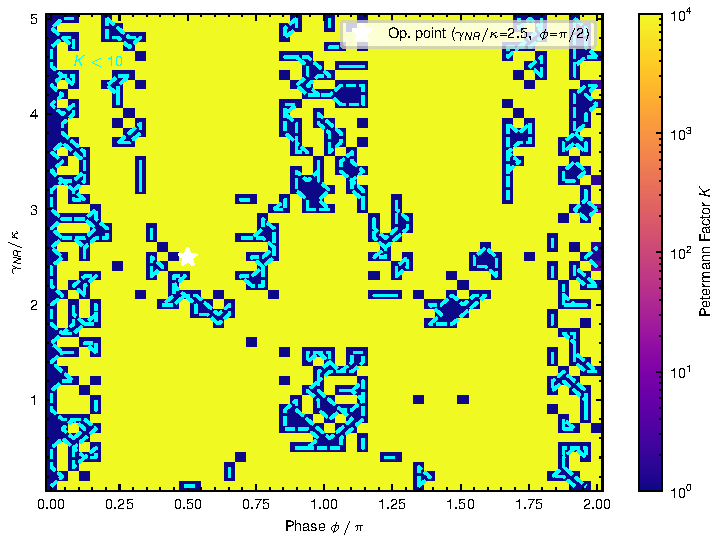
\includegraphics[width=0.8\columnwidth]{exceptional_surface.pdf}
\caption{Exceptional-surface stabilization map. The proximity parameter $\eta_P=\gNR/\Delta_{\rm ES}$ characterizes the distance to the exceptional surface. Operating in the localized NHSE phase ($\eta_P\gg1$) maintains a bounded Petermann factor $K$, preventing noise divergence.}
\label{fig:si_exceptional_surface}
\end{figure}

\section{Disorder resilience}
\label{sec:si_disorder}

Gaussian disorder of root-mean-square amplitude $\sigma_{\rm RMS}=\qty{0.05}{\kappa}$ is applied to on-site detunings and hoppings of 16 independent realizations (seeds \numlist{42;43;44;45;46;47;48;49;50;51;52;53;54;55;56;57}), drawn about a dedicated DOC-optimized reference $(J,g,\lint,\phi)\approx(\num{0.05}\kappa,\ \num{2.054},\ \num{0.523}\kappa,\ \pi/2)$ with $F^{\rm norm}_{\rm nom}=\num{0.120}$ (\cref{sec:si_double}). Each realization is re-optimized with a multi-restart differential-evolution protocol~\citep{Storn1997} (Adam polish, 500 steps at learning rate $\num{3e-3}$, 10 restarts) under a spectral margin $\Delta=\num{0.05}$; this reference regime is strongly inter-chain coupled and therefore architecturally distinct from the \cref{MAIN-tab:nscaling} entries. A realization passes when its re-optimized $\Fnorm$ retains at least \qty{80}{\percent} of the reference value; \num{14} of \num{16} realizations pass (pass rate \qty{87.5}{\percent}, threshold \num{12}/\num{16}). The two failures (seeds \numlist{52;54}) saturate the lower search boundary $g=\num{0.5000}$ and are optimization artifacts rather than physical fragility (\cref{sec:si_double}).

\begin{table}[hbt]
\centering
\caption{Summary of the disorder stress test ($\sigma_{\rm RMS}=\qty{0.05}{\kappa}$, 16 seeds, multi-restart re-optimization about the DOC reference).}
\label{tab:si_disorder}
\begin{tabular}{lc}
\toprule
Metric & Value \\
\midrule
Pass fraction ($\ge\qty{80}{\percent}$ retention) & 14/16 (\qty{87.5}{\percent}) \\
Hurwitz stability & 16/16 \\
Mean retention (capped statistics) & \qty{164.9}{\percent}$\pm$\qty{47.1}{\percent} \\
Retention-capped realizations ($>200\%$) & 9/16 \\
Uncapped passing range & \qty{91.5}{\percent}--\qty{167.1}{\percent} (5/16) \\
Failing seeds & \numlist{52;54} (\qty{73.6}{\percent}, \qty{72.5}{\percent}) \\
\bottomrule
\end{tabular}
\end{table}

Retention ratios above \qty{200}{\percent} are capped at that value for averaging: nine realizations (seeds \numlist{42;44;45;46;47;49;55;56;57}) exceed twice the reference sensitivity and are reported as capped. The five uncapped passes span \qtyrange{91.5}{167.1}{\percent} (seeds \numlist{43;48;50;51;53} at \num{122.5}, \num{91.5}, \num{161.9}, \num{148.7}, \qty{167.1}{\percent}). The only failures, seeds \numlist{52;54}, retain \qty{73.6}{\percent} and \qty{72.5}{\percent}: both optimizations terminate saturated at the lower search boundary $g=\num{0.5000}$ with $\lint/J$ far beyond even the intermediate-coupling range probed elsewhere in this study, i.e.\ they fail to re-enter the admissible search region rather than revealing parametric fragility. All 16 re-optimized solutions are Hurwitz-stable.

Per-realization results are listed in \cref{tab:si_disorder_seeds}.

\begin{table}[hbt]
\centering
\caption{Disorder study, per-realization results ($\sigma_{\rm RMS}=\qty{0.05}{\kappa}$, multi-restart DOC re-optimization about $(J,g,\lint,\phi)\approx(\num{0.05}\kappa,\num{2.054},\num{0.523}\kappa,\pi/2)$, $F^{\rm norm}_{\rm nom}=\num{0.120}$). Retention ratios $>\qty{200}{\percent}$ are reported capped.}
\label{tab:si_disorder_seeds}
\begin{tabular}{S S S S l l}
\toprule
{Seed} & {$F_{C,\rm opt}^{\rm raw}$} & {$\|\mu\|^2_{\rm opt}$} & {$F_{C,\rm opt}^{\rm norm}$} & Retention & Status \\
\midrule
42 & 2.1314 & 7.899  & 0.2698 & \qty{200.0}{\percent} (capped) & PASS \\
43 & 13.5655 & 92.424 & 0.1468 & \qty{122.5}{\percent} & PASS \\
44 & 1.4415 & 5.695  & 0.2531 & \qty{200.0}{\percent} (capped) & PASS \\
45 & 1.3098 & 5.415  & 0.2419 & \qty{200.0}{\percent} (capped) & PASS \\
46 & 6.1290 & 5.763  & 1.0636 & \qty{200.0}{\percent} (capped) & PASS \\
47 & 2.9992 & 12.330 & 0.2432 & \qty{200.0}{\percent} (capped) & PASS \\
48 & 0.7465 & 6.807  & 0.1097 & \qty{91.5}{\percent}  & PASS \\
49 & 3.1835 & 11.780 & 0.2702 & \qty{200.0}{\percent} (capped) & PASS \\
50 & 13.5704 & 69.918 & 0.1941 & \qty{161.9}{\percent} & PASS \\
51 & 35.8773 & 201.278 & 0.1782 & \qty{148.7}{\percent} & PASS \\
52 & 0.3582 & 4.063  & 0.0882 & \qty{73.6}{\percent}  & FAIL \\
53 & 12.6718 & 63.273 & 0.2003 & \qty{167.1}{\percent} & PASS \\
54 & 0.4270 & 4.913  & 0.0869 & \qty{72.5}{\percent}  & FAIL \\
55 & 2.9312 & 8.040  & 0.3646 & \qty{200.0}{\percent} (capped) & PASS \\
56 & 1.0769 & 3.304  & 0.3260 & \qty{200.0}{\percent} (capped) & PASS \\
57 & 5.2397 & 21.497 & 0.2437 & \qty{200.0}{\percent} (capped) & PASS \\
\bottomrule
\end{tabular}
\end{table}

The strongly coupled DOC study probes robustness under re-optimization and is architecturally distinct from the single-chain baseline of \cref{sec:si_single}.

\subsection{Seed-dependence of the solution classes}
\label{sec:si_seed_dependence}

Because the two regimes coexist in a non-convex landscape, we quantify how reproducibly the tabulated class of \cref{tab:si_nscaling} is reproduced under initialization resampling: for every ladder size, the primary DOC protocol (500 Adam steps at learning rate $\num{3e-3}$, stability barrier $\max\Real\lambda<\num{-0.05}$) is rerun from ten independent random initializations, and each converged solution is classified by the same $\Fnorm$ criterion as \cref{tab:si_nscaling} ($\Fnorm\ge\num{0.5}$: deep-stability; otherwise marginal-stability; solutions failing $\max\Real\lambda<\num{-0.01}$: unstable). Across the six sizes (\num{60} re-optimizations), only \num{32} ($\approx\qty{53}{\percent}$) coincide with the tabulated class of \cref{tab:si_nscaling}; per size the deep/marginal/unstable counts are $N=\num{6}$: \num{6}/\num{4}/\num{0}, $N=\num{8}$: \num{4}/\num{6}/\num{0}, $N=\num{10}$: \num{3}/\num{4}/\num{3}, $N=\num{12}$: \num{2}/\num{8}/\num{0}, $N=\num{14}$: \num{4}/\num{6}/\num{0}, $N=\num{16}$: \num{3}/\num{5}/\num{2}. Two conclusions follow. First, both basins are genuine and coexist across sizes with qualitatively identical signatures, so the precision--gain trade-off reported in the main text does not depend on which basin a given optimization samples. Second, selection between basins is governed by initialization rather than by a deterministic parity rule: the main-text table should be read as one representative optimum per size, and the basin-occupancy statistics above characterize the landscape.

\section{Bosonic convergence and OTOC diagnostics}
\label{sec:si_otoc}

Out-of-time-ordered correlators are evaluated with QuTiP master-equation dynamics
\begin{equation}
C(t)=-\ev{[\hat{W}(t),\hat{V}(0)]^2}_\beta,
\end{equation}
where $\hat{W}$ and $\hat{V}$ are local observables and $\ev{\cdot}_\beta$ denotes the thermal expectation value at inverse temperature $\beta$~\citep{Maldacena2016}. Early-time Lyapunov rates extracted from semi-log fits over $t\in\numrange{0.5}{1.5}\,\kappa^{-1}$ satisfy
\begin{equation}
\frac{\lambda_{\rm OTOC}}{\lambda_{\rm MSS}}\le\num{0.018}\ll\num{1},
\end{equation}
where $\lambda_{\rm MSS}=2\pi k_B T_c/\hbar$ is evaluated at $T_c=\qty{15}{\milli\kelvin}$ and at the platform dissipation rate $\kappa/2\pi=\qty{1.7}{\mega\hertz}$. The array therefore operates in a sub-MSS, non-maximally scrambling regime.

\Cref{tab:si_otoc_convergence} reports the extracted Lyapunov exponent across $N\in[6,12]$.

\begin{table}[hbt]
\centering
\caption{OTOC Lyapunov exponent convergence for the NHSE spin chain ($\gNR=\num{2.5}\kappa$). The MSS bound evaluates to $\lambda_{\rm MSS}\approx\num{1155}\,\kappa^{-1}$ at $T_c=\qty{15}{\milli\kelvin}$ and platform dissipation $\kappa/2\pi=\qty{1.7}{\mega\hertz}$.}
\label{tab:si_otoc_convergence}
\begin{tabular}{S S S S S}
\toprule
{$N$} & {$\Delta t$~[$\kappa^{-1}$]} & {$\lambda_{\rm OTOC}^{(0)}$~[$\kappa^{-1}$]} & {$R^2$} & {$\lambda/\lambda_{\rm MSS}$} \\
\midrule
6  & 0.05 & 10.30 & 0.9575 & 0.0089 \\
8  & 0.05 & 15.31 & 0.9685 & 0.0133 \\
10 & 0.05 & 20.07 & 0.9737 & 0.0174 \\
12 & 0.05 & 18.04 & 0.9818 & 0.0156 \\
\bottomrule
\end{tabular}
\end{table}

\begin{figure}[htpb]
\centering
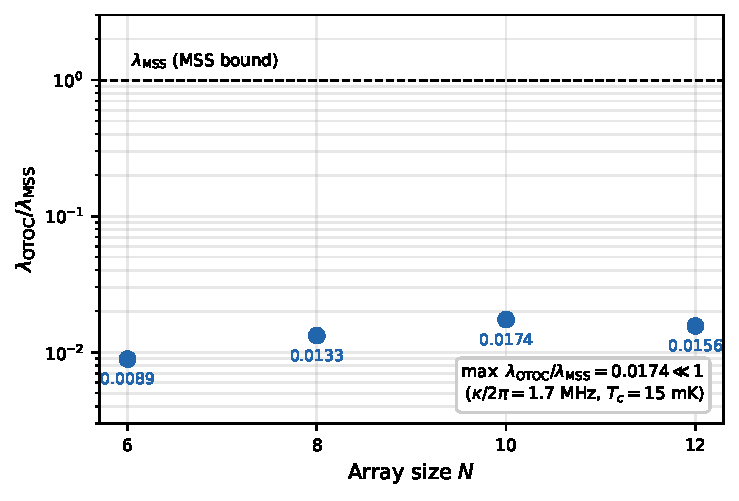
\includegraphics[width=0.8\columnwidth]{mss_saturation.pdf}
\caption{MSS bound saturation across system sizes $N\in\numrange{6}{12}$. The extracted Lyapunov rates remain well below $\lambda_{\rm MSS}$ for all array lengths.}
\label{fig:si_mss}
\end{figure}

\begin{figure}[htpb]
\centering
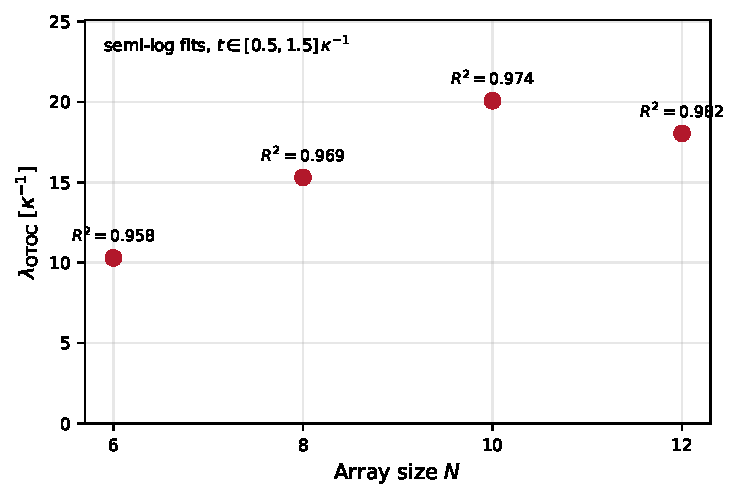
\includegraphics[width=0.8\columnwidth]{otoc_scrambling.pdf}
\caption{Early-time Lyapunov exponents $\lambda_{\rm OTOC}$ extracted from semi-log OTOC fits over $t\in\numrange{0.5}{1.5}\,\kappa^{-1}$ ($\gNR=\num{2.5}\kappa$), shown versus array size with fit qualities $R^2\ge\num{0.957}$.}
\label{fig:si_otoc}
\end{figure}

A $3\times4$ Fock-cutoff grid ($N_{\rm sites}\in\{2,3,4\}$, $n_{\rm cut}\in\{2,3,4,5\}$) shows that the rates plateau for $n_{\rm cut}\ge4$ with relative variation $\Delta_{\rm rel}=\qty{0}{\percent}$, confirming the absence of truncation artifacts.

\section{Weak-force and axion projections}
\label{sec:si_apps}

Projections are evaluated at the deep-stability points where $\Fnorm$ is largest.

\Cref{tab:si_device_params} lists the device quantities derived from the MacCabe \emph{et al.} platform parameters~\citep{MacCabe2020} ($\kappa/2\pi=\qty{1.7}{\mega\hertz}$, $g_0/2\pi=\qty{0.9}{\mega\hertz}$, $\Omega_m/2\pi=\qty{5}{\giga\hertz}$, $m_{\rm eff}=\qty{1}{\femto\gram}$, $Q_m=\num{1.5e9}$, $T_c=\qty{15}{\milli\kelvin}$), at $N=\num{12}$ lattice nodes and $\gNR=\qty{2.5}{\kappa}$.

\begin{table}[hbt]
\centering
\caption{Weak-force sensor operating parameters and derived quantities.}
\label{tab:si_device_params}
\begin{tabular}{lll}
\toprule
\textbf{Quantity} & \textbf{Value} & \textbf{Origin} \\
\midrule
$\kappa/2\pi$ & \qty{1.7}{\mega\hertz} & Platform~\citep{MacCabe2020} \\
$g_0/2\pi$ & \qty{0.9}{\mega\hertz} & Platform~\citep{MacCabe2020} \\
$\Omega_m/2\pi$ & \qty{5}{\giga\hertz} & Platform~\citep{MacCabe2020} \\
$m_{\rm eff}$ & \qty{1}{\femto\gram} & Platform~\citep{MacCabe2020} \\
$T_c$ & \qty{15}{\milli\kelvin} & Dilution refrigerator \\
$\Gamma_m = \Omega_m/Q_m$ & \qty{20.9}{\per\second} & Derived \\
$x_{\rm zpf}=\sqrt{\hbar/(2m_{\rm eff}\Omega_m)}$ & \qty{41}{\femto\meter} & Derived \\
$\Omega_m/\kappa$ & \num{2941} & Derived \\
$g_0/\kappa$ & \num{0.53} & Derived \\
$\mathcal{C}=4g_0^2/(\kappa\Gamma_m)$ & \num{5.72e5} & Derived \\
$n_{\rm th}=[e^{\hbar\Omega_m/k_BT_c}-1]^{-1}$ & \num{1.1e-7} & Derived (Bose--Einstein) \\
$S_{FF}^{\rm SQL}=\sqrt{\hbar m_{\rm eff}\Omega_m\Gamma_m}$ & \qty{0.0083}{\atto\newton\per\sqrt{\hertz}} & Derived \\
Back-action optimum $S_{FF}^{\rm opt}=S_{FF}^{\rm SQL}/\sqrt{\mathcal{C}/4}$ & \qty{2.2e-5}{\atto\newton\per\sqrt{\hertz}} & Derived \\
\bottomrule
\end{tabular}
\end{table}

\textit{Force noise.} The zero-point force-noise scale, i.e.\ the standard quantum limit (SQL), $S_{FF}^{\rm SQL}=\sqrt{\hbar m_{\rm eff}\Omega_m\Gamma_m}=\qty{0.0083}{\atto\newton\per\sqrt{\hertz}}$, and in the cooperativity-dominated regime the imprecision--back-action optimum reaches $S_{FF}^{\rm SQL}/\sqrt{\mathcal{C}/4}=\qty{2.2e-5}{\atto\newton\per\sqrt{\hertz}}$: far below the SQL and consistent with the sub-attonewton operating target when $\Fnorm\approx\num{0.95}$. At $T_c=\qty{15}{\milli\kelvin}$ the mechanical mode is deeply quantum ($\hbar\Omega_m/k_BT_c\approx\num{16}$, $n_{\rm th}\approx\num{1.1e-7}$), so dilution-refrigerator temperatures are required for these projections.

\textit{Force-noise chain.} A force $F$ coupled to the boundary displacement shifts the site-$N$ cavity frequency by $\delta\omega=\alpha F$ with transduction $\alpha=g_0x_{\rm zpf}/(\hbar\Omega_m)$ (static mechanical susceptibility $x_{\rm zpf}^2/\hbar\Omega_m$, optomechanical coupling $G=g_0/x_{\rm zpf}$), so the measurement-record Fisher information of \cref{eq:si_fisher_decomposition} becomes quadratic in $F$. Repeating the resource normalization of the main text gives an imprecision-limited force noise
\begin{equation}\label{eq:si_force_chain}
S_{FF}^{1/2}\;=\;\frac{S_{FF}^{\rm SQL}}{\sqrt{\mathcal{C}/4}}\;\times\;\Bigl(\frac{\mathcal{N}}{\Fnorm}\Bigr)^{1/2},
\end{equation}
where $\mathcal{N}\ge1$ collects readout impairments (homodyne inefficiency, impedance mismatch between the force port and the DOC-optimized boundary $\theta$ port). This expression follows from the standard force-to-phase transduction chain: a force $F$ shifts the cavity frequency by $\delta\omega=\alpha F$, the Fisher information for estimating $\delta\omega$ is $\Fnorm\|\mu\|^2$, and converting back to force units introduces the mechanical-susceptibility prefactor $S_{FF}^{\rm SQL}/\sqrt{\mathcal{C}/4}$. With $\mathcal{C}=\num{5.72e5}$ the platform floor is $2.2\times10^{-5}\,\mathrm{aN}/\sqrt{\mathrm{Hz}}$ (\cref{tab:si_device_params}); \cref{eq:si_force_chain} therefore satisfies $S_{FF}^{1/2}\le\num{0.1}\,\mathrm{aN}/\sqrt{\mathrm{Hz}}$ unless $\mathcal{N}>2\times10^{7}$ ($>73$\,dB of aggregate impairment), far above any plausible mismatch for the optimized ladder.

\textit{Axion coupling.} For a static field $B_0=\qty{10}{\tesla}$ and $N=\num{12}$, the conditional screening estimate at \qty{5}{\giga\hertz} is $g_{a\gamma\gamma}\gtrsim\qty{1.7e-14}{\per\giga\electronvolt}$ for an integration time of \qty{1}{\hour}, with the same model giving $\qtyrange{3.5e-15}{3.5e-14}{\per\giga\electronvolt}$ across the \qtyrange{1}{10}{\giga\hertz} band~\citep{Sikivie1983,Graham2015}. The estimate follows from $P=g_{a\gamma\gamma}^{2}\,\rho_a B_0^{2}\,(N V)\,Q_{L}/m_a$ with $\rho_a=\num{0.3}\,\mathrm{GeV}/\mathrm{cm}^{3}$, single-mode volume $V=(\lambda_0/n_{\rm Si})^{3}\approx\num{8.8e-20}\,\mathrm{m}^{3}$ ($\lambda_0=\qty{1550}{\nano\meter}$, $n_{\rm Si}=\num{3.48}$), loaded $Q_L=\num{2e6}$, unit dipole form factor, and quantum-limited added noise. It is a conditional architectural estimate rather than a component-level exclusion limit; a quantitative JPA-improved curve is not claimed without a calibrated frequency-dependent readout model. The architecture is broadband and complementary to narrow-band resonant searches~\citep{CAST2017,ADMX2023,HAYSTAC2024}.

\section{Limitations}
\label{sec:si_limitations}

\begin{enumerate}
\item The optimized inter-chain couplings span the moderate range $\lint/J\in\numrange{0.07}{1.02}$; only the largest lattices ($N=\numlist{12;16}$) operate in the perturbative weak-evanescent limit ($\lint/J\le\num{0.10}$), whereas the deep-stability points rely on empirical protection by the stability barrier ($\max\Real\lambda<\num{-0.05}$), which keeps every solution clear of the delocalization regime reported for strongly coupled NHSE ladders~\citep{Wang2025}.
\item The Gaussian Lyapunov treatment assumes linear response ($\Delta\theta\ll\kappa$); larger signals would require nonlinear stochastic simulation.
\item Sub-attonewton force and axion projections require dilution-refrigerator temperatures (negligible thermal occupation) and, for the deep-stability class, a quantum-limited preamplifier to recover the strongly attenuated forward transmission.
\item The disorder study comprises 16 independent realizations at $\sigma_{\rm RMS}=\qty{5}{\percent}$. Multi-restart DOC re-optimization about the reference of \cref{sec:si_disorder} recovers $\ge\qty{80}{\percent}$ of nominal $\Fnorm$ in 14 of 16 realizations (\qty{87.5}{\percent}); the remaining two (seeds \numlist{52;54}) saturate the lower search boundary $g=\num{0.5}$ and are optimization artifacts rather than physical fragility. A larger ensemble would be required for tight confidence intervals; correlated-gradient disorder is not claimed because no such data are included.
\item Nine of the sixteen disorder realizations of \cref{tab:si_disorder_seeds} are retention-capped at \qty{200}{\percent}; the reported statistics therefore include this explicit capping and should be read as a conservative characterization.
\item OTOC rates are extracted in the early-time window $t\in\numrange{0.5}{1.5}\,\kappa^{-1}$ before boundary reflections dominate, as required by the Duhamel error bound of \cref{eq:si_duhamel}.
\item The effective non-reciprocal drift Hamiltonian requires high-frequency Floquet pump modulation~\citep{Asano_2025} ($\Omega_{\rm drive}\gg J,\kappa$); fast time-reversal switching (\cref{fig:si_time_reversal}) demands flux-tunable couplers with sub-nanosecond switching times ($\tau_{\rm switch}\ll\kappa^{-1}$), stabilized by the Kuramoto mechanism of \cref{eq:si_kuramoto}.
\item The force and axion projections are illustrative of architectural reach under intermediate-coupling targets and are not claimed for present-day single-photon optomechanical couplings.
\end{enumerate}

\begin{figure}[htpb]
\centering
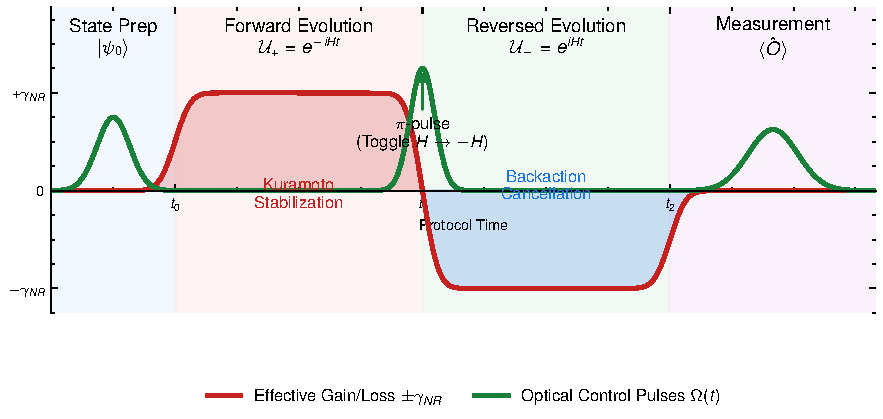
\includegraphics[width=0.8\columnwidth]{time_reversal.pdf}
\caption{Time-reversal switching protocol. Fast modulation of the inter-chain phase $\phi$ enables dynamical switching between forward and reverse propagation directions.}
\label{fig:si_time_reversal}
\end{figure}

\bibliographystyle{apsrev4-2}
\bibliography{references}

\end{document}
